\documentclass[11pt,a4paper]{article}

% --- Language and Fonts ---
\usepackage[T1]{fontenc}
\usepackage[utf8]{inputenc}
\usepackage[spanish]{babel} % Standard Spanish support [cite: 2]
\usepackage{csquotes} % for proper quotation marks [cite: 3]

% --- Sans-serif font (global) ---
\usepackage{lmodern}     % Latin Modern fonts
\renewcommand{\familydefault}{\sfdefault}

% --- Math and Symbols ---
\usepackage{amsmath, amssymb, amsfonts}

% --- Layout and Graphics ---
\usepackage[margin=2.5cm]{geometry}
\usepackage{graphicx}
\usepackage{booktabs} 
\usepackage{longtable}
\usepackage{hyperref}
\usepackage{placeins} % for \FloatBarrier command [cite: 13]

% Set path to images (one level up) [cite: 14]
\graphicspath{{../figures/}}

% --- Bibliography ---
\usepackage[backend=biber, style=authoryear]{biblatex}
\addbibresource{references.bib}

% Custom Spanish month-year date format for frontpage
\newcommand{\monthyeardate}{%
  \ifcase\month\or
    Enero\or Febrero\or Marzo\or Abril\or Mayo\or Junio\or
    Julio\or Agosto\or Septiembre\or Octubre\or Noviembre\or Diciembre\fi
  \space\number\year
}

% Metadata

\title{MapBiomas Argentina Fuego \\ \large Proyecto Piloto}
\author{Iván Barberá}
\date{\today}


%%%%%%%%%%%%%%%%%%%%%%%%%%%%%%%%%%%%%%%

\begin{document}

\begin{titlepage}
\thispagestyle{empty}

\vspace*{1cm}

\begin{center}

% --- Logo ---

\includegraphics[width=0.65\textwidth]{logo_mapbiomas_fuego.png}

\vspace{1.5cm}

% --- Project ---
{\Large \textbf{MapBiomas Argentina Fuego}}\\[1.0cm]

% --- Main title ---
{\Large \textbf{ATBD}}\\[0.3cm]

{\large \textit{Algorithm Theoretical Basis Document}}\\[0.5cm]


% --- Collection and version ---
{\large Proyecto piloto}\\[0.3cm]
{\large Version 1.0}\\[2cm]

% --- Coordination ---
{\large \textbf{Coordinador general}}\\[0.3cm]
Iván Barberá\\[1.0cm]

% --- Team ---
{\large \textbf{Equipo}}\\[0.3cm]
\begin{tabular}{@{}l l@{}}
Camilo Bagnato          & Daniela Arpigiani \\
Lican Martínez          & Micaela Abrigo \\
Ramón Peña Agrest       & Juan Gowda \\
Gonzalo Dieguez Gaviola & Leónidas Lizárraga \\
Ana Eljall              & Mariana Lipori \\
Luna Schteingart        & Nehuen Bedeti \\
José Daniel Lencinas   & Fabio Trinco \\
Pablo Baldassini       & Andrés Leszczuk \\
Juan Argañaraz         & Tomás Vujanic \\
Santiago Verón         & Thomas Kitzberger \\
Fernando Salvaré       & Dalma Raymundi \\
Camila Mateo           & Roxana Gimenez \\
Micaela Gambino        & Gabriela Nicosia
\end{tabular}
\vfill


% --- Date ---
{\large \monthyeardate}

\end{center}

\end{titlepage}

\tableofcontents

\newpage

\section{Introducción}

\subsection{Alcance y propósito del documento}

Este documento describe las bases teóricas, el marco metodológico y las consideraciones operativas utilizadas para desarrollar el piloto de MapBiomas Argentina Fuego. El piloto no constituye una colección oficial de MapBiomas; sin embargo, su estructura, conceptos y flujos de trabajo están diseñados para ser la base metodológica de la Colección 1 de MapBiomas Argentina Fuego para el año 2026.

\subsection{Objetivos del piloto}

Los objetivos de este piloto fueron

\begin{itemize}
  \item conformar un grupo de trabajo capaz de elaborar mapas de área quemada para integrarlas en una colección de MapBiomas Argentina, y
  \item desarrollar un algoritmo de mapeo que presente una precisión razonable, con una demanda relativamente baja de recursos humanos para la toma de muestras de entrenamiento.
\end{itemize}

Particularmente, buscamos generar los mismos productos de área quemada ofrecidos por MapBiomas Brasil Fuego en su \href{https://plataforma.brasil.mapbiomas.org/fire/fire_total_burned?tl[id]=4&tl[themeKey]=fire&tl[subthemeKey]=fire_total_burned&tl[legendKey]=fire_total_burned_mapbiomas_total_burned&tl[year]=2024&tl[pixelValues][]=1&t[regionKey]=brazil&t[ids][]=1-1-1&t[divisionCategoryId]=4}{plataforma}, a saber: capa anual de área quemada con mes de quema y tamaño de la cicatriz; capa de frecuencia de fuego, y capa de año del último incendio \parencite{alencar2022mapbiomas_fire}.

\subsection{Extensión espacial y temporal del piloto}

Como área piloto escogimos una porción de la Patagonia argentina, abarcando un marcado gradiente de productividad: al oeste se encuentran los bosques andino-patagónicos, y al este, la estepa patagónica (Fig.~\ref{fig-area-piloto}), abarcando un área de $182104 \ \text{km}^2$. Por su variada productividad, esta región presenta desafíos que se extenderán en otras regiones del país, a saber: disturbios que afectan a los bosques, como defoliaciones y tala; incendios de sotobosque que son difíciles de detectar, y zonas afectadas por sequías o zonas de muy baja productividad que se confunden con áreas quemadas.

Dado que previo a 1998 en la región de interés la cobertura de imágenes Landsat es casi nula, decidimos mapear el período 1999--2025. No incluimos 1998 porque el algoritmo actual requiere de imágenes en el año anterior al que se desea mapear.

\begin{figure}[ht]
  \centering
  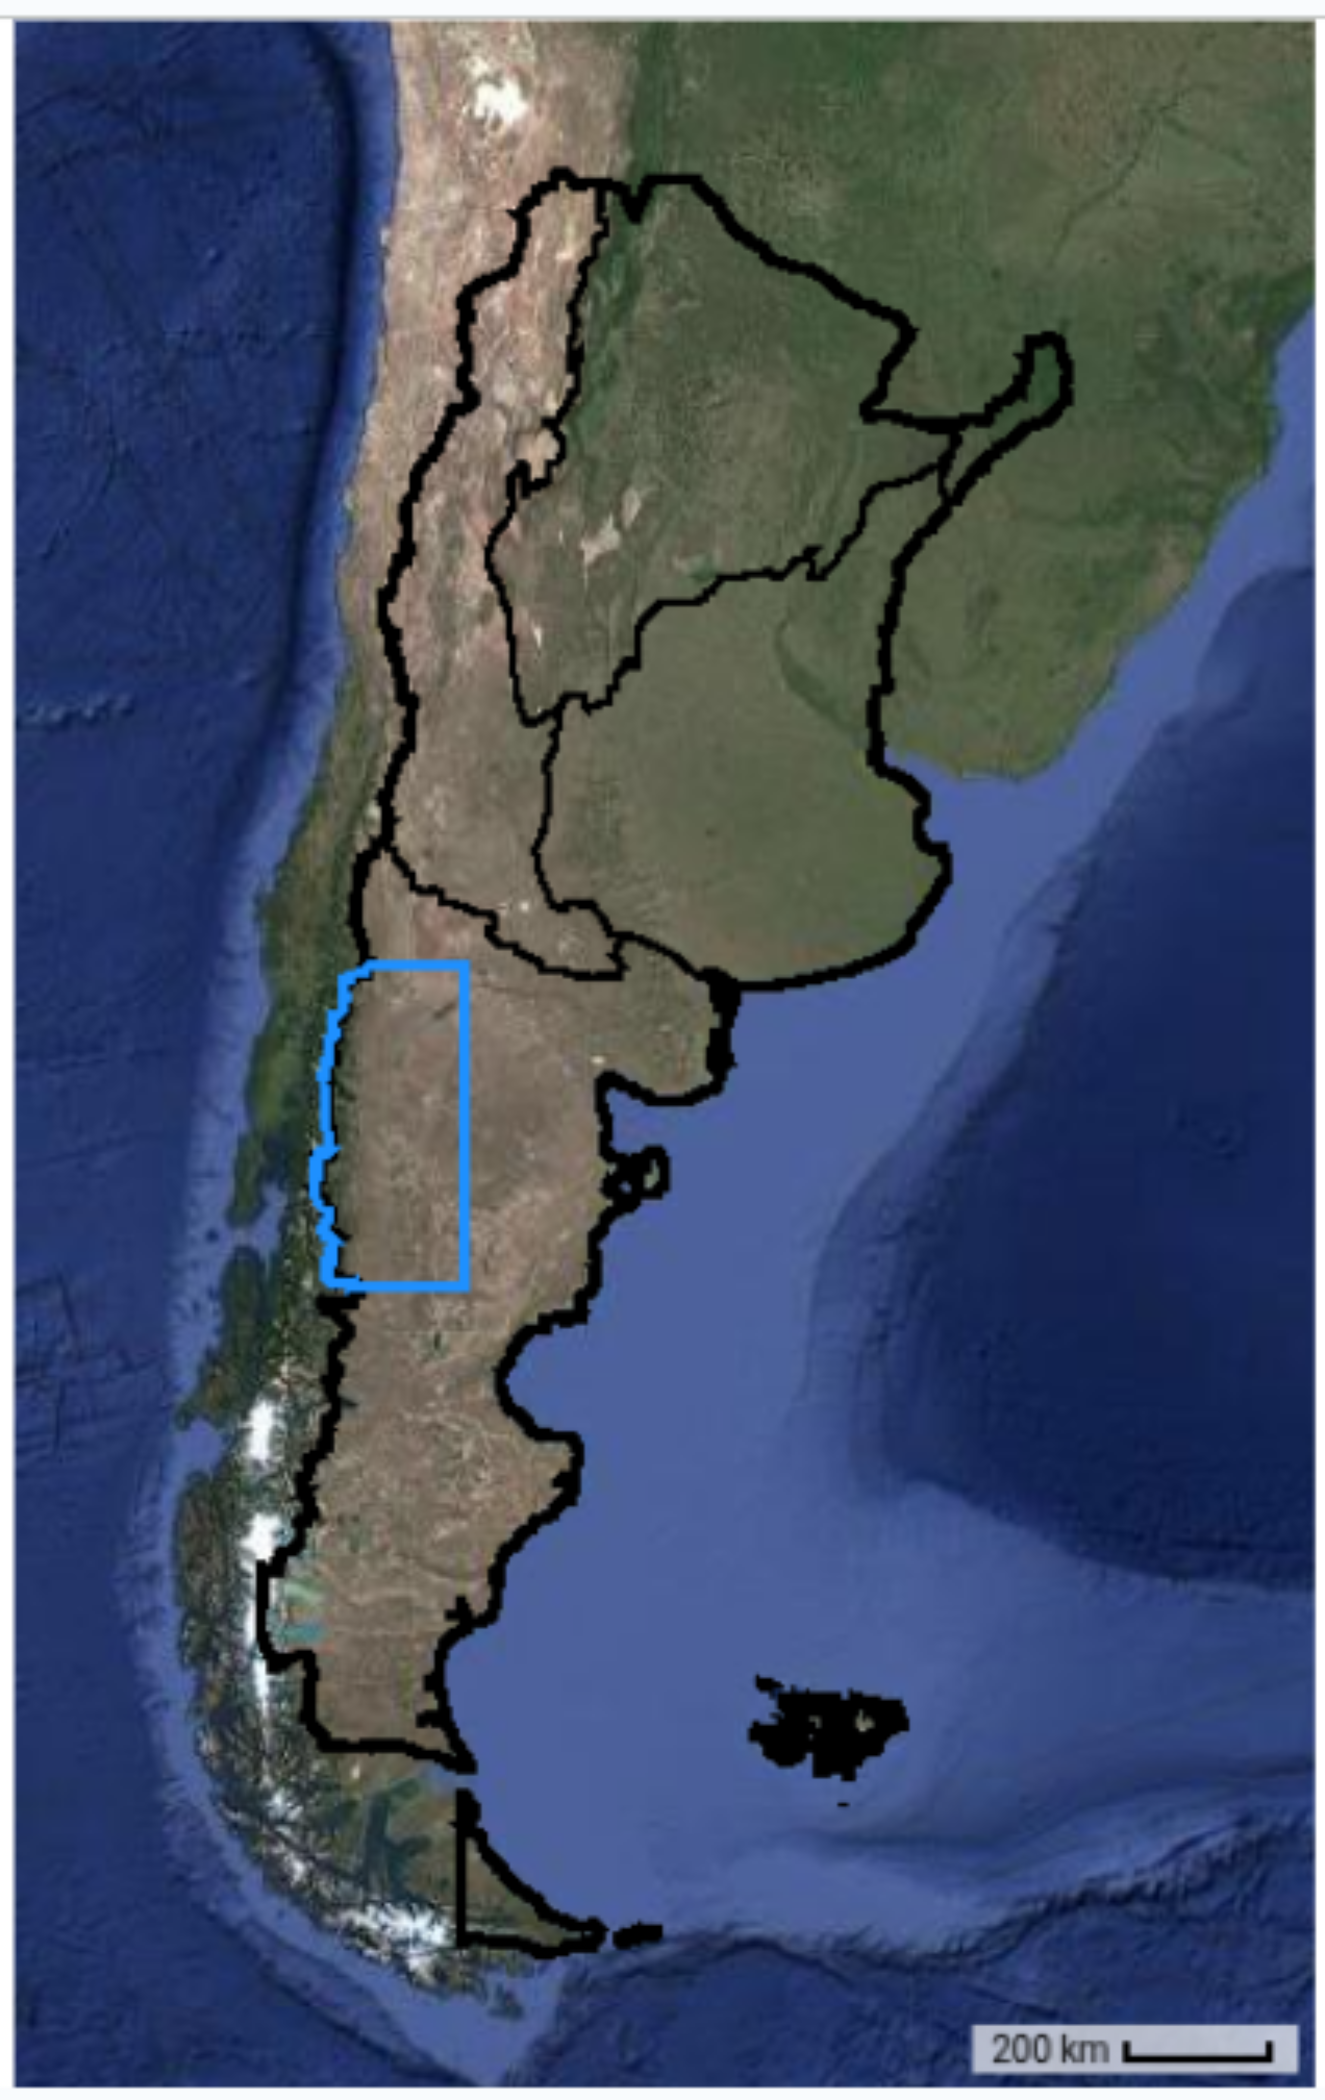
\includegraphics[width=0.45\textwidth]{area_piloto.png}
  \caption{Área piloto del proyecto (celeste), y las 5 regiones definidas por MapBiomas Argentina (negro).}
  \label{fig-area-piloto}
\end{figure}

\FloatBarrier

\subsection{Bases de datos utilizadas}

El piloto de MapBiomas Argentina Fuego se desarrolló utilizando series temporales completas de imágenes Landsat y capas auxiliares de MapBiomas Argentina, procesadas íntegramente en Google Earth Engine (GEE; \citeauthor{gorelick_google_2017}~\citeyear{gorelick_google_2017}).

\subsubsection{Imágenes Landsat}

Se utilizaron todas las imágenes disponibles de Landsat Colección 2 (30 m de resolución) Nivel 2 (Surface Reflectance) que intersectan el área de estudio y el período 1998--2025 \parencite{landsatc2}. A partir de 1999 se dispone de cobertura temporal suficiente para el análisis, mientras que 1998 se empleó únicamente como año previo de referencia para el cálculo de métricas interanuales.

Durante el período de estudio estuvieron activos los siguientes sensores Landsat:

\begin{itemize}
  \item \textbf{Landsat 5 TM} (1984--2013),
  \item \textbf{Landsat 7 ETM+} (1999--presente),
  \item \textbf{Landsat 8 OLI} (2013--presente),
  \item \textbf{Landsat 9 OLI-2} (2021--presente).
\end{itemize}

Las bandas consideradas fueron azul (BLUE), verde (GREEN), rojo (RED), infrarrojo cercano (NIR) e infrarrojo de onda corta 1 y 2 (SWIR1, SWIR2), ya que estas bandas permiten calcular índices espectrales sensibles al fuego y a cambios en la cobertura vegetal.

\subsubsection{Filtros de calidad}

Las imágenes Landsat fueron filtradas utilizando la banda QA\_PIXEL provista en los productos de reflectancia de superficie de la Colección 2. Se excluyeron observaciones afectadas por nubes, nubes dilatadas, sombras de nubes, nieve y agua.

No se aplicaron interpolaciones temporales ni rellenos espaciales, por lo que la densidad de observaciones varía espacial y temporalmente según la disponibilidad de imágenes libres de nubes.

\subsubsection{Armonización espectral entre sensores}

Dado que la serie temporal combina sensores con respuestas espectrales ligeramente diferentes, se aplicó un procedimiento de armonización espectral para asegurar la comparabilidad entre observaciones de distintos sensores. En particular, las reflectancias de Landsat 5 TM y Landsat 7 ETM+ fueron transformadas al dominio espectral de Landsat 8/9 OLI, utilizando los coeficientes estimados por \textcite{roy2016harmonization}.

Este procedimiento se aplicó banda a banda sobre las reflectancias de superficie, luego de la conversión a unidades físicas, y permite reducir discontinuidades artificiales en las series temporales asociadas al cambio de sensor. Las imágenes OLI y OLI-2 no fueron transformadas.

\subsubsection{Capa de cobertura y uso del suelo de MapBiomas}

Como información auxiliar se utilizó la clasificación de cobertura y uso del suelo de MapBiomas Argentina Colección 2, región Patagonia \parencite{mapbiomasarg}, con resolución espacial de 30 m y cobertura anual, reclasificada en tres tipos amplios de vegetación: bosque, arbustal y pastizal, además de la clase no quemable que fue enmascarada.

El tipo de vegetación se utilizó para ajustar modelos probabilísticos separados por clase, y para restringir el análisis a superficies quemables. En todos los casos se utilizó la clasificación correspondiente al año previo al año focal, con el objetivo de evitar inconsistencias introducidas por cambios en la cobertura causados por el mismo incendio que se desea detectar. La reclasificación de la capa original de MapBiomas se describe en el Cuadro~\ref{tab-remapeo-clases}.

\begin{table}[ht]
\centering
\caption{Remapeo de clases de cobertura y uso del suelo de MapBiomas Argentina (Colección 2) a clases funcionales para el mapeo de incendios.}
\label{tab-remapeo-clases}
\begin{tabular}{l c l c}
\toprule
Clase MapBiomas & ID MapBiomas & Clase fuego & ID fuego \\
\midrule
Bosque cerrado          & 3  & Bosque      & 1 \\
Arbustal                & 66 & Arbustal    & 2 \\
Leñosas inundables      & 6  & Bosque      & 1 \\
Pastizales              & 12 & Pastizal    & 3 \\
Humedales               & 11 & Pastizal    & 3 \\
Turberas                & 75 & Pastizal    & 3 \\
Estepa                  & 63 & Pastizal    & 3 \\
Mosaico de usos         & 21 & Pastizal    & 3 \\
Plantaciones forestales & 9  & Bosque      & 1 \\
Roca altoandina         & 29 & No quemable & 0 \\
Desiertos y eriales     & 25 & No quemable & 0 \\
Áreas urbanas           & 24 & No quemable & 0 \\
Ríos, lagos y océano    & 33 & No quemable & 0 \\
Glaciares, nieve y hielo& 34 & No quemable & 0 \\
No observado            & 27 & No quemable & 0 \\
\bottomrule
\end{tabular}
\end{table}

\subsection{Plataformas de cómputo}

La mayor parte del piloto fue ejecutada en GEE, que además de ofrecer un notable poder de cómputo en la nube, almacena todo el archivo Landsat y los productos de MapBiomas. El entrenamiento de los modelos de clasificación se llevó a cabo localmente, utilizando el lenguaje R \parencite{R}, pero sus predicciones fueron calculadas enteramente en GEE.

\section{Algoritmo de mapeo de áreas quemadas}

El algoritmo consta de dos grandes bloques, en los cuales se considera (1) el contexto temporal, mediante análisis de series temporales, y (2) el contexto espacial, mediante un algoritmo de crecimiento de región y filtros a nivel de objetos (Fig.~\ref{fig-algo}).

\begin{figure}[ht]
  \centering
  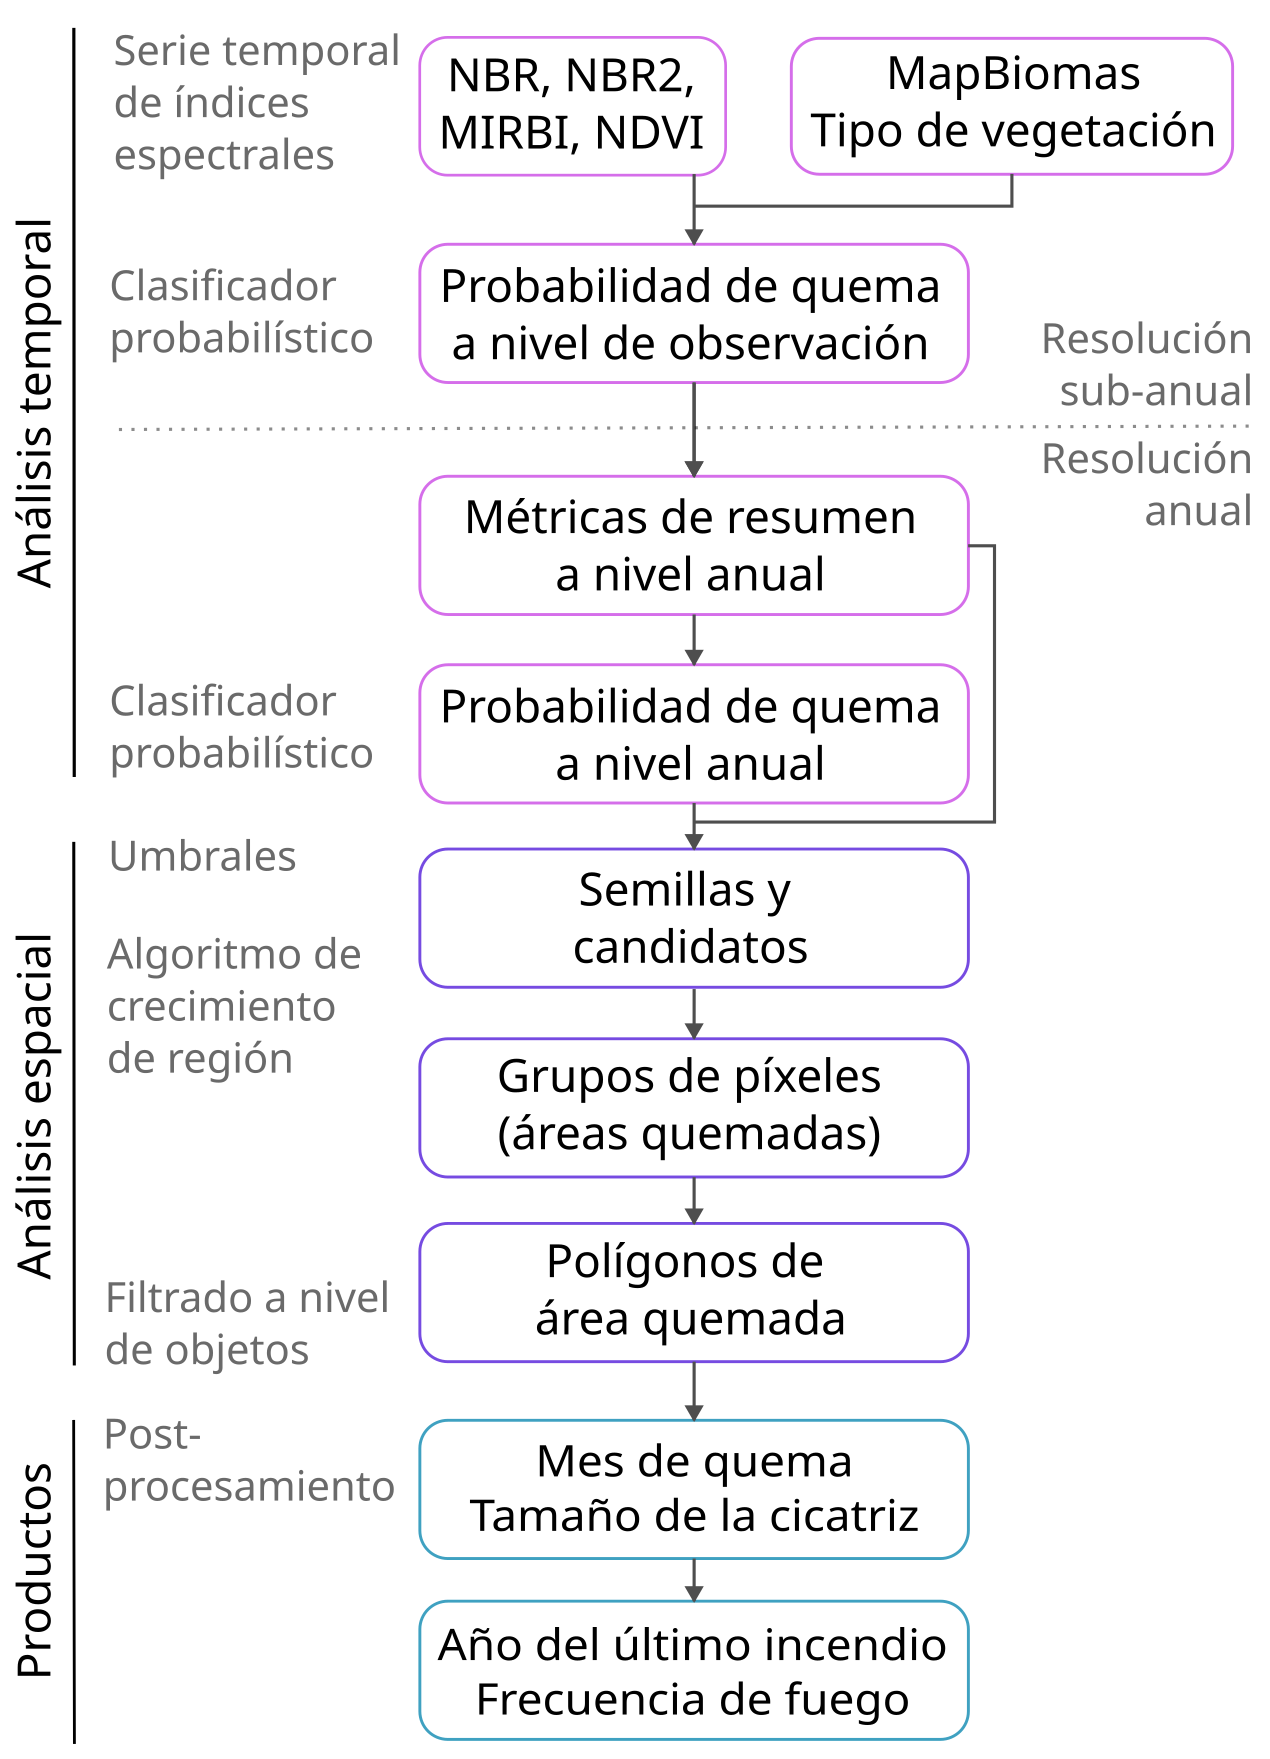
\includegraphics[width=0.5\textwidth]{algoritmo.png}
  \caption{Algoritmo de mapeo de áreas quemadas.}
  \label{fig-algo}
\end{figure}

\FloatBarrier

\subsection{Análisis temporal}

Dado que el fuego genera cambios en la señal espectral, la primera etapa del algoritmo consiste de un detector de cambio orientado a la detección de áreas quemadas. En una primera etapa se transforma la señal espectral en probabilidad de quema a nivel de observación de Landsat (píxel-fecha), mediante un clasificador probabilístico entrenado con datos (Fig.~\ref{fig-ts-example}A y \ref{fig-ts-example}B). Esto arroja una serie temporal de probabilidad de quema por píxel, de la cual se obtienen métricas de resumen anuales, como la máxima probabilidad de quema y su máximo aumento entre observaciones consecutivas (Fig.~\ref{fig-ts-example}C). Posteriormente, estas métricas de resolución anual se utilizan para obtener la probabilidad de quema a nivel anual, mediante otro clasificador probabilístico (Fig.~\ref{fig-ts-example}D).

\subsubsection{Probabilidad de quema a nivel de observación}

Un enfoque sencillo para clasificar una observación (píxel-fecha) como quemado / no quemado implica determinar un umbral de algún índice espectral sensible al fuego. Por ejemplo, se puede establecer un umbral de NBR o de dNBR. Sin embargo, este esquema sencillo es poco generalizable porque el umbral óptimo varía entre tipos de vegetación (e.g., bosque-pastizal), y también varía según la productividad, estructura y composición de la vegetación, incluso dentro de un mismo tipo de vegetación. A su vez, utilizar más de un índice espectral suele aumentar la precisión, ya que algunos incendios generan cambios en algunos índices espectrales pero no en otros (e.g., las zonas poco productivas no muestran un marcado descenso del NIR, por lo que índices basados en bandas SWIR suelen ser más efectivos). Estas consideraciones han llevado a que generalmente se opte por modelos de clasificación multivariados, es decir, que toman muchas variables predictoras para clasificar las observaciones en quemado o no quemado. Algunos ejemplos de modelos son árboles de decisión, random forest, support vector machines, redes neuronales y regresión logística. En particular, aquellos modelos que devuelven la probabilidad de cada clase, denominados clasificadores probabilísticos, permiten considerar la incertidumbre asociada a la clasificación.

Dado que nuestro objetivo fue generar una serie temporal de probabilidad de quema a nivel de observación, requeríamos calcular esta probabilidad predicha por un modelo en cada imagen Landsat intersectando el área y período de estudio. Debido al alto costo computacional de esta operación, escogimos la regresión logística, que permite calcular la probabilidad de quema a muy bajo costo. Además, al ser un modelo de estructura sencilla, puede implementarse fácilmente en GEE, lo cual permite escalar su evaluación a un gran volumen de datos.

\paragraph{Variables predictoras a nivel de observación}

Como variables predictoras de la regresión logística utilizamos cuatro índices espectrales sensibles al fuego: NBR \parencite{key_benson_2006}, NBR2 \parencite{usgs_landsat_burned_area_2021}, MIRBI \parencite{trigg_flasse_2001} y NDVI \parencite{tucker_1979}, definidos de la siguiente manera:

\begin{equation*}
  \begin{aligned}
    \mathrm{NBR} &= \frac{\mathrm{NIR} - \mathrm{SWIR2}}{\mathrm{NIR} + \mathrm{SWIR2}} \\
    \\
    \mathrm{NBR2} &= \frac{\mathrm{SWIR1} - \mathrm{SWIR2}}{\mathrm{SWIR1} + \mathrm{SWIR2}} \\
    \\
    \mathrm{MIRBI} &= (10 \cdot \mathrm{SWIR2} - 9.8 \cdot \mathrm{SWIR1} + 2) \cdot (-1)\\
    \\
    \mathrm{NDVI} &= \frac{\mathrm{NIR} - \mathrm{RED}}{\mathrm{NIR} + \mathrm{RED}}\text{,}
  \end{aligned}
\end{equation*}

\noindent donde la multiplicación del MIRBI por $-1$ responde a conveniencias operativas, ya que de esta manera los cuatro índices disminuyen tras el paso del fuego.

Además, incluimos en el modelo tres variables derivadas de estos índices. Utilizamos el mínimo y máximo valor del año anterior al focal para caracterizar la productividad y estacionalidad de la vegetación, y utilizamos la diferencia mínimo previo - valor focal para detectar cambio en la señal espectral.

Definimos el mínimo y máximo anual de una forma robusta a valores extremos. Sea $\{ \mathrm{INDEX}_j \}_{j=1}^{N}$ el conjunto de observaciones válidas anuales de un índice espectral a nivel de píxel, ordenadas de menor a mayor, definimos los estimadores robustos de mínimo y máximo anual como:

\begin{equation}
  \begin{aligned}
    \mathrm{INDEX}_L &=
    \begin{cases}
      \frac{1}{2}\left( \mathrm{INDEX}_{(2)} + \mathrm{INDEX}_{(3)} \right), & \text{si } N > 20 \\
      \frac{1}{2}\left( \mathrm{INDEX}_{(1)} + \mathrm{INDEX}_{(2)} \right), & \text{si } 9 \le N \le 20 \\
      \mathrm{INDEX}_{(1)}, & \text{si } 2 \le N < 9 \\
      \mathrm{NA}, & \text{si } N < 2
    \end{cases} \\
    \\
    \mathrm{INDEX}_H &=
    \begin{cases}
      \frac{1}{2}\left( \mathrm{INDEX}_{(N-1)} + \mathrm{INDEX}_{(N-2)} \right), & \text{si } N > 20 \\
      \frac{1}{2}\left( \mathrm{INDEX}_{(N)} + \mathrm{INDEX}_{(N-1)} \right), & \text{si } 9 \le N \le 20 \\
      \mathrm{INDEX}_{(N)}, & \text{si } 2 \le N < 9 \\
      \mathrm{NA}, & \text{si } N < 2
    \end{cases}
  \end{aligned}
  \label{eq-min-max}
\end{equation}

Utilizamos el mínimo para calcular la diferencia entre el mínimo del año anterior y cada observación en el año focal:

\[ \mathrm{INDEX}_{\Delta,t} = \mathrm{INDEX}_{L,y(t)-1} - \mathrm{INDEX}_{t}, \]

\noindent donde $t$ representa cada observación en el año focal, y el sufijo $y(t)-1$ indica el año anterior al cual corresponde la observación $t$.

Como la función de probabilidad de quema puede ser distinta entre tipos de vegetación, ajustamos una regresión logística separada para cada tipo (bosque, arbustal y pastizal; ver Cuadro~\ref{tab-remapeo-clases}). La capa de vegetación utilizada para generar la predicción fue la del año anterior al focal, ya que la clasificación del año focal podría estar alterada por el mismo fuego que se desea detectar.

De esta manera, para cada observación (píxel-fecha) se utilizaron los cuatro índices registrados en la fecha correspondiente, sus valores $\Delta$ basados en el mínimo del año anterior, el mínimo y máximo del año anterior de cada índice y la capa de vegetación del año anterior, reclasificada.

\paragraph{Estructura del modelo}

La regresión logística define la probabilidad de la observación correspondiente al píxel $c$ y al momento $t$ corresponda a quemado [$\Pr(\text{y}_{c,t} = 1)$] de la siguiente manera:

\begin{equation}
  \label{eq-logistic}
  \begin{aligned}
    \Pr(\text{y}_{c,t} = 1) &= \frac{1}{1 + \exp(-\eta_{c,t})} \\
    \eta_t &= \alpha_{k[c]} + \sum_{j=1}^J \beta_{j,k[c]} x_{j,c,t},
  \end{aligned}
\end{equation}

\noindent donde $\alpha$ y $\beta$ son parámetros a estimar, el subíndice $k \in \{1, 2, 3\}$ representa el tipo de vegetación, y la notación $k[c]$ indica el tipo de vegetación correspondiente al pixel $c$ en el año previo al que corresponde el momento $t$. $J = 40$ es la cantidad de términos de regresión. Las $x_j$ representaban variables crudas y términos de interacción (productos), listados a continuación.

\vspace{1em}

Efectos principales de índices focales:
\[
\begin{aligned}
&\mathrm{NBR},\;
\mathrm{NBR2},\;
\mathrm{MIRBI},\;
\mathrm{NDVI}
\end{aligned}
\]

Efectos principales de mínimo y máximo anual previo:
\[
\begin{aligned}
&\mathrm{NBR}_L,\;
\mathrm{NBR}_H,\;
\mathrm{NBR2}_L,\;
\mathrm{NBR2}_H,\;
\mathrm{MIRBI}_L,\;
\mathrm{MIRBI}_H,\;
\mathrm{NDVI}_L,\;
\mathrm{NDVI}_H
\end{aligned}
\]

Interacciones índice–min/max anual:
\[
\begin{aligned}
&\mathrm{NBR} \times \mathrm{NBR}_L,\;
\mathrm{NBR} \times \mathrm{NBR}_H,\;
\mathrm{NBR}_L \times \mathrm{NBR}_{\Delta},\;
\mathrm{NBR}_H \times \mathrm{NBR}_{\Delta}, \\
&\mathrm{NBR2} \times \mathrm{NBR2}_L,\;
\mathrm{NBR2} \times \mathrm{NBR2}_H,\;
\mathrm{NBR2}_L \times \mathrm{NBR2}_{\Delta},\;
\mathrm{NBR2}_H \times \mathrm{NBR2}_{\Delta}, \\
&\mathrm{MIRBI} \times \mathrm{MIRBI}_L,\;
\mathrm{MIRBI} \times \mathrm{MIRBI}_H,\;
\mathrm{MIRBI}_L \times \mathrm{MIRBI}_{\Delta},\;
\mathrm{MIRBI}_H \times \mathrm{MIRBI}_{\Delta}, \\
&\mathrm{NDVI} \times \mathrm{NDVI}_L,\;
\mathrm{NDVI} \times \mathrm{NDVI}_H,\;
\mathrm{NDVI}_L \times \mathrm{NDVI}_{\Delta},\;
\mathrm{NDVI}_H \times \mathrm{NDVI}_{\Delta}
\end{aligned}
\]

Interacciones entre índices (valores focales):
\[
\begin{aligned}
&\mathrm{NBR} \times \mathrm{NBR2},\;
\mathrm{NBR} \times \mathrm{MIRBI},\;
\mathrm{NBR} \times \mathrm{NDVI}, \\
&\mathrm{NBR2} \times \mathrm{MIRBI},\;
\mathrm{NBR2} \times \mathrm{NDVI},\;
\mathrm{MIRBI} \times \mathrm{NDVI}
\end{aligned}
\]

Interacciones entre diferencias:
\[
\begin{aligned}
&\mathrm{NBR}_{\Delta} \times \mathrm{NBR2}_{\Delta},\;
\mathrm{NBR}_{\Delta} \times \mathrm{MIRBI}_{\Delta},\;
\mathrm{NBR}_{\Delta} \times \mathrm{NDVI}_{\Delta}, \\
&\mathrm{NBR2}_{\Delta} \times \mathrm{MIRBI}_{\Delta},\;
\mathrm{NBR2}_{\Delta} \times \mathrm{NDVI}_{\Delta},\;
\mathrm{MIRBI}_{\Delta} \times \mathrm{NDVI}_{\Delta}.
\end{aligned}
\]

Los parámetros del modelo fueron estimados por máxima verosimilitud, suponiendo una distribución Bernoulli de la variable respuesta (0: no quemado, 1: quemado).

\paragraph{Datos de entrenamiento}\label{sec-prob-obs}

Seleccionamos 30 incendios detectados por MODIS en el período 2001-2025. Escogimos 15 incendios en la franja oeste del área de estudio, dominada por bosques andino-patagónicos, con baja abundancia de arbustales y pastizales, y 15 incendios situados al este, en la región dominada por la estepa patagónica, con baja abundancia de bosques y arbustales. En cada incendio definimos períodos pre-fuego y post-fuego, donde se evidenciaba señal de quema en imágenes Landsat. Basados en el falso color post-fuego, tomamos aproximadamente 200 puntos quemados y 200 puntos no quemados por incendio, intentando abarcar la mayor variabilidad espectral posible en cada clase, recurriendo a la evaluación visual de series temporales de índices espectrales en las zonas de clasificación dudosa.

Con este procedimiento obtuvimos un total de 12889 puntos. Para entrenar el modelo a nivel de observación extrajimos la serie temporal de índices espectrales en cada punto, utilizando todas las observaciones disponibles de imágenes Landsat. Los puntos quemados aportaron ceros a partir de su período prefuego (no quemado), y unos (quemado) a partir de su período post-fuego. Los puntos no quemados, sólo aportaron ceros.

Al utilizar como datos de entrenamiento la serie temporal de observaciones extraída en cada punto, ajustamos el modelo con $589797$ observaciones. Es decir, en promedio, cada punto muestreado aportó $45.76$ observaciones. De esas $589797$ observaciones, $99414$ ($16.86$ \%) fueron etiquedas como quemado, y $490383$, como no quemado. 

Nuestra estrategia de muestreo aprovecha al máximo el esfuerzo dedicado a seleccionar puntos. Si cada punto aporta $45.76$ observaciones, un análisis superficial indicaría que su eficacia es mayor a la de tomar más muestras extrayendo una única observación por punto, en un factor de $45.76$. Sin embargo, dado que las observaciones extraídas en un mismo punto están correlacionadas temporalmente, la ganancia real es menor. Pero esto no es un problema en sí, ya que de todos modos nuestro método requiere series temporales por punto para el modelo a nivel anual (ver Sección~\ref{sec-prob-anual}). Aun así, para extraer series temporales de los puntos se requiere definir periodos pre- y post-fuego por incendio, lo cual demanda un esfuerzo mayor a sólo definir el año de quema. Nuestra recolección de incendios (30 eventos) tomó un total de $5.10$ h, mientras que la recolección de muestras una vez definidos los incendios tomó $35.97$ h, siendo el tiempo total dedicado $41.07$ h. Para comparar con el método de extraer una sola observación por punto, suponemos que el tiempo de recolección de incendios se reduciría a un $20$ \% ($1.02$ h), por no requerir definir precisos períodos pre- y post-fuego. Bajo este supuesto, para extraer tantas observaciones como las que obtuvimos, se requerirían $589797$ puntos, lo cual tomaría un total de $1645.98$ h. Sumando $1.02$ h de recolección de incendios, resultaría en $1647.00$ h ($68.63$ días). Este valor supera a nuestro esfuerzo de muestreo por un factor de $40.10$. Es decir, nuestro enfoque puede multiplicar la eficiencia por $40$.

\subsubsection{Probabilidad de quema a nivel anual}\label{sec-prob-anual}

Dado que MapBiomas produce mapas de resolución temporal anual, se requiere un resultado a nivel anual. Para obtener tal producto, resumimos la serie temporal de probabilidad de quema en métricas anuales. Sin embargo, las series temporales de índices espectrales presentan ruido, en parte debido a que los filtros de calidad de Landsat presentan cierto grado de error. Para evitar que el ruido generase falsos positivos, antes de resumir la serie en cada píxel, la suavizamos, utilizando la mediana de $K = 5$ observaciones, asignando la observación a la fecha central. De esta manera, para que un fuego sea detectado con probabilidad alta, la misma debe presentar valores elevados durante al menos tres observaciones. Definimos $K = 5$ mediante prueba y error, visualizando series temporales crudas y suavizadas, variando $K$. Notamos que en años con baja densidad de imágenes (e.g., pre 2000), suavizar con $K = 5$ podía generar errores de omisión, ya que con observaciones muy separadas en el tiempo, la señal de quema puede desaparecer en menos de tres observaciones. Una mejora a futuro sería utilizar una ventana de suavizado dinámica, definida en base a la cantidad de observaciones en el año, a nivel de píxel.

Dado que en muchas regiones la estación de incendios cruza el año calendario, como en Patagonia, y que los incendios pueden transcurrir entre el fin de un año y el comienzo del siguiente, corríamos el riesgo de omitir incendios ocurridos en el fin o comienzo del año. Para evitar este problema aplicamos una estrategia redundante: antes de suavizar la serie temporal de probabilidad de quema de un año, le añadimos $M = 4$ observaciones del año previo y del posterior, permitiendo $M - 2$ observaciones extra en la serie suavizada. Si bien este paso genera áreas quemadas duplicadas en años consecutivos, los duplicados fueron removidos en un paso posterior.

\paragraph{Métricas de resumen a nivel anual}

A partir de la serie temporal suavizada de probabilidad de quema en cada año, calculamos las siguientes métricas, a nivel de píxel y con resolución anual:

\begin{itemize}
  \item pmax: máxima probabilidad de quema,
  \item pdiff\_max: máxima diferencia consecutiva en probabilidad de quema,
  \item Pmax: máxima probabilidad de quema acumulada,
  \item Pdiff\_max: máxima diferencia consecutiva en probabilidad de quema acumulada,
  \item date\_pre: fecha de la observación que precede al máximo aumento en probabilidad de quema,
  \item date\_post: fecha de la observación en que la probabilidad de quema presentó el mayor aumento.
  \item date\_mid: fecha intermedia entre date\_pre y date\_post.
\end{itemize}

Las fechas fueron almacenadas como año fraccional. 
La probabilidad de quema acumulada hasta la observación $t$ es la probabilidad de que al menos una observación en la serie suavizada se observe como quemada hasta el tiempo $t$, y se define de la siguiente manera:

Sea $\{ p_t \}_{t=1}^{T}$ la serie temporal de probabilidad de quema a nivel de observación para todo un año en un píxel, obtenida a partir del clasificador probabilístico y, suavizada mediante la mediana de 5 observaciones.

La probabilidad de quema acumulada hasta la observación $t$, definida como la probabilidad de que al menos una observación corresponda a quemado hasta dicho tiempo, se calcula como:

\[
P_t = 1 - \prod_{i=1}^{t} \left( 1 - p_i \right).
\]

Incluimos esta métrica porque en quemas de baja severidad la probabilidad no llega a valores muy altos, pero se observan muchas observaciones con probabilidad intermedia, lo cual podría reflejarse mejor en este valor acumulado.

\paragraph{Clasificador probabilístico a nivel anual}

Para obtener una probabilidad de quema a nivel anual ajustamos una segunda regresión logística. En este caso, incluimos como predictoras las siguientes variables:

\vspace{1em}

Métricas de probabilidad de quema

\[
\begin{aligned}
&\text{pmax},\;
\text{pdiff\_max},\;
\text{Pmax},\;
\text{Pdiff\_max}
\end{aligned}
\]

Interacciones entre métricas de probabilidad

\[
\begin{aligned}
&\text{pmax} \times \text{pdiff\_max},\;
\text{pmax} \times \text{Pmax},\;
\text{pmax} \times \text{Pdiff\_max}, \\
&\text{pdiff\_max} \times \text{Pmax},\;
\text{pdiff\_max} \times \text{Pdiff\_max},\;
\text{Pmax} \times \text{Pdiff\_max}
\end{aligned}
\]

Índices espectrales del año previo

\[
\begin{aligned}
&\mathrm{NBR}_L,\;
\mathrm{NBR}_H,\;
\mathrm{NBR2}_L,\;
\mathrm{NBR2}_H,\;
\mathrm{MIRBI}_L,\;
\mathrm{MIRBI}_H,\;
\mathrm{NDVI}_L,\;
\mathrm{NDVI}_H
\end{aligned}
\]

Interacciones entre índices espectrales del año previo

\[
\begin{aligned}
&\mathrm{NBR}_L \times \mathrm{NBR}_H,\;
\mathrm{NBR}_L \times \mathrm{NBR2}_L,\;
\mathrm{NBR}_L \times \mathrm{NBR2}_H,
\mathrm{NBR}_L \times \mathrm{MIRBI}_L,\\
&\mathrm{NBR}_L \times \mathrm{MIRBI}_H,\;
\mathrm{NBR}_L \times \mathrm{NDVI}_L,
\mathrm{NBR}_L \times \mathrm{NDVI}_H, 
\mathrm{NBR}_H \times \mathrm{NBR2}_L,\\
&\mathrm{NBR}_H \times \mathrm{NBR2}_H,\;
\mathrm{NBR}_H \times \mathrm{MIRBI}_L,\;
\mathrm{NBR}_H \times \mathrm{MIRBI}_H,\;
\mathrm{NBR}_H \times \mathrm{NDVI}_L,\\
&\mathrm{NBR}_H \times \mathrm{NDVI}_H, 
\mathrm{NBR2}_L \times \mathrm{NBR2}_H,\;
\mathrm{NBR2}_L \times \mathrm{MIRBI}_L,\;
\mathrm{NBR2}_L \times \mathrm{MIRBI}_H,\\
&\mathrm{NBR2}_L \times \mathrm{NDVI}_L,\;
\mathrm{NBR2}_L \times \mathrm{NDVI}_H, 
\mathrm{NBR2}_H \times \mathrm{MIRBI}_L,\;
\mathrm{NBR2}_H \times \mathrm{MIRBI}_H,\\
&\mathrm{NBR2}_H \times \mathrm{NDVI}_L,\;
\mathrm{NBR2}_H \times \mathrm{NDVI}_H, 
\mathrm{MIRBI}_L \times \mathrm{MIRBI}_H,\;
\mathrm{MIRBI}_L \times \mathrm{NDVI}_L,\\
&\mathrm{MIRBI}_L \times \mathrm{NDVI}_H,\;
\mathrm{MIRBI}_H \times \mathrm{NDVI}_L,\;
\mathrm{MIRBI}_H \times \mathrm{NDVI}_H, 
\mathrm{NDVI}_L \times \mathrm{NDVI}_H.
\end{aligned}
\]

Al igual que en el caso anterior, los parámetros fueron estimados por máxima verosimilitud, definiendo un modelo separado para cada tipo de vegetación.

\begin{figure}[ht]
  \centering
  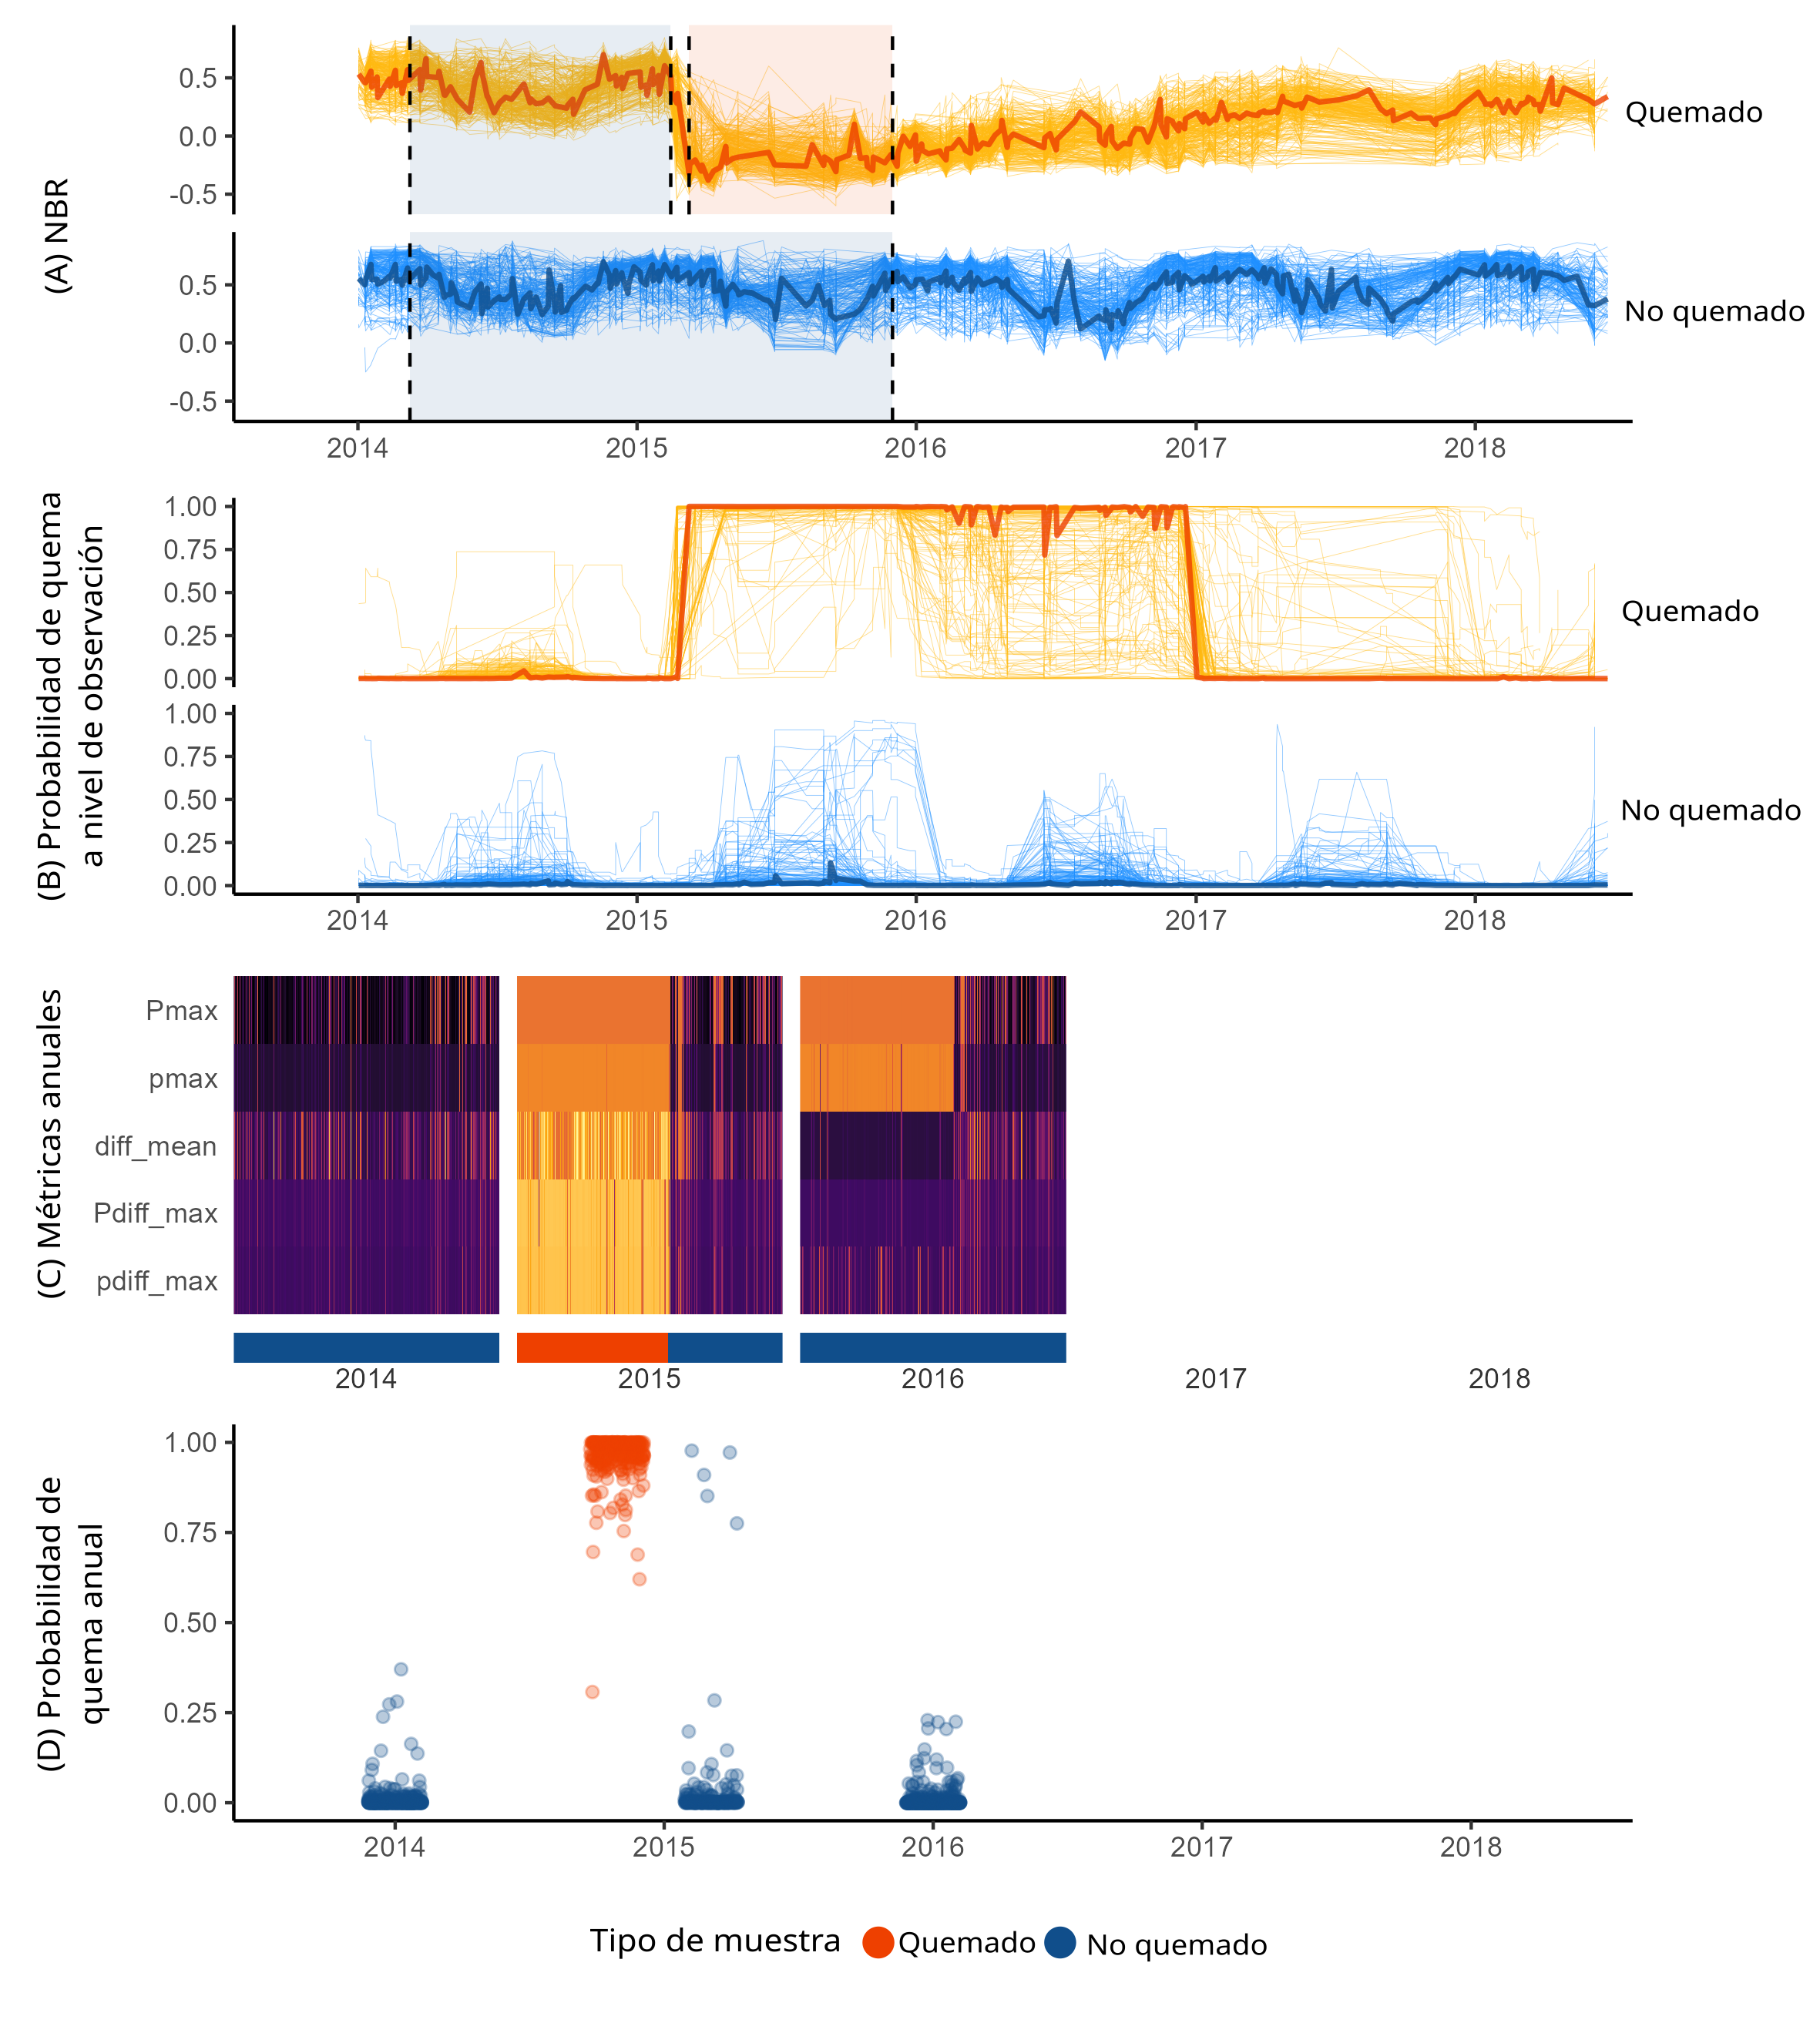
\includegraphics[width=\textwidth]{tempSegPlot_n5_fire_01_spanish.png}
  \caption{Análisis temporal para puntos de entrenamiento muestreados en el incendio de Cholila (2015). (A) Serie temporal de NBR. Las líneas verticales discontinuas delimitan los perídos pre- y post-fuego en los puntos quemados, y en el caso de los puntos no quemados, delimitan el rango de fechas utilizado para extraer observaciones de la clase no quemado. (B) Probabilidad de quema a nivel de observación obtenida mediante el clasificador probabilístico. Las líneas delgadas en (A) y (B) representan la serie en los puntos de entrenamiento, mientras que las líneas gruesas representan la mediana entre observaciones, includa aquí sólo con fines gráficos. (C) Métricas anuales derivadas de la serie temporal de probabilidad de quema. El mapa de calor presenta valores más claros en registros que presentan valores más altos. (D) Probabilidad de quema a nivel anual obtenida mediante el segundo clasificador probabilístico. Los años pre- y post-fuego (2014 y 2016) sólo aportan datos de la clase no quemado.}
  \label{fig-ts-example}
\end{figure}

\FloatBarrier

\paragraph{Datos de entrenamiento}

Para ajustar el modelo a nivel anual utilizamos la misma base de datos obtenida para el modelo a nivel de observación. Al obtener las series de índices espectrales, extrajimos datos de aproximadamente cuatro años alrededor del incendio. Esto permitió obtener datos a nivel anual. Sobre la serie temporal de cada punto se calculó la probabilidad de quema a nivel de observación, la misma fue suavizada, y se obtuvieron métricas anuales. Posteriormente, a estas observaciones anuales se las etiquetó como quemadas si correspondían al año del fuego y a un punto quemado, y como no quemadas si alguna de estas dos condiciones no se cumplía. De esta manera, a partir de los $12889$ puntos muestreados, obtuvimos $38047$ registros a nivel anual, de los cuales, $7671$ ($20.16$ \%) correspondieron a la clase quemado.

Si bien en este caso no extrajimos tantas observaciones por punto como en el modelo a nivel de observación (Sección~\ref{sec-prob-obs}), por cada punto muestreado obtuvimos $38047 / 12889 = 2.95$ observaciones a nivel anual. Para lograr este aumento en la eficiencia de toma de datos, sólo se requiere utilizar datos provenientes de zonas quemadas y no quemadas en donde no hayan ocurrido incendios en los años adyacentes. Con esa restricción, que no implica definir períodos precisos pre- y post-fuego, podemos suponer que el tiempo de recolección de incendios se reduciría a un $50$ \% del tiempo que invertimos, es decir, $5.1 / 2 = 2.55$ h. De esta manera, para obtener $38047$ observaciones a nivel anual, extrayendo un sólo registro por punto, se requeriría un total de $108.69$ h. En este caso, nuestro método, con $41.07$ h dedicadas, muestra una eficiencia mayor, en un factor de $2.64$. En regiones con baja incidencia del fuego es sencillo encontrar zonas no quemadas en años adyacentes, incluso en ventanas mayores a tres años, con lo cual, la eficiencia de muestreo se podría aumentar aún más. Esta estrategia puede ser de utilidad en esquemas de mapeo donde las muestras de entrenamiento se toman a nivel anual, como en MapBiomas Fuego Brasil \parencite{alencar2022mapbiomas_fire}.  

\subsection{Análisis espacial}

Este segundo bloque del algoritmo de detección de áreas quemadas explota el hecho de que los incendios generan cambios espectrales en grupos contiguos de píxeles, no como eventos aislados. Este bloque incluye tres pasos: segmentación espacial mediante un algoritmo de crecimiento de región, mascareo mediante polígonos definidos manualmente, y filtrado a nivel de objetos (Fig.~\ref{fig-algo} y \ref{fig-region-growing}). 

\subsubsection{Algoritmo de crecimiento de región}

Si bien un clasificador a nivel anual puede clasificar cada píxel como quemado o no quemado, los clasificadores probabilísticos nos permiten explotar la incertidumbre sobre la clasificación. Los algoritmos de crecimiento de región generan grupos de celdas contiguas que cumplen cierta característica \parencite{adams_bischof_1994,haralick_shapiro_1985}. En el contexto de mapeo de áreas quemadas, estos algoritmos han sido ampliamente utilizados para expandir detecciones confiables hacia píxeles espectralmente ambiguos, explotando la naturaleza espacialmente contagiosa del fuego \parencite{fraser2000,giglio2009,hawbaker2020,long2019}.

Para aplicar el crecimiento de región, es necesario definir capas binarias de semillas y candidatos. Las semillas son píxeles con alta probabilidad de estar quemados, y los candidatos, aquellos donde la probabilidad es menor. En la primera iteración, cada semilla conforma un grupo de celdas, y en cada iteración subsecuente se agregan a estos grupos todos los píxeles candidatos que se encuentran en el vecindario de ocho celdas. Al finalizar el procedimiento, los candidatos no conectados con algún grupo son enmascarados.

Este procedimiento permite explotar un compromiso favorable entre errores de comisión (clasificar quemado lo que no está quemado) y omisión (clasificar no quemado lo que sí está quemado). Las semillas tienen alto error de omisión, pero bajo error de comisión; los candidatos, lo opuesto. A su vez, al definir estas capas se pueden añadir otros filtros que no hayan sido incorporados en la probabilidad de quema (e.g., \citeauthor{long2019}~\citeyear{long2019}).

Definimos la capa de semillas como el conjunto de píxeles que cumplen:

\[
\text{semilla} =
\left\{
\begin{array}{l}
\text{pmax} \ge 0.98, \\
\text{pdiff\_max} \ge 0.90, \\
\text{pannual} \ge 0.98, \\
\mathrm{bright}_H \le 0.5 \;\land\;
\mathrm{bright}_{\Delta} \le 0.15,
\end{array}
\right.
\]

\noindent con $\text{pmax}$ y $\text{pdiff\_max}$ definidos previamente, y siendo $\text{pannual}$ la probabilidad de quema a nivel anual. La última condición corresponde a un filtro de brillo diseñado para prevenir la identificación de semillas en áreas afectadas por ceniza volcánica u otras superficies altamente reflectivas no asociadas a fuego.

En particular, $\mathrm{bright}_H$ representa el valor máximo anual, en el año focal, del componente de brillo derivado de la transformación \textit{Tasseled Cap} de Landsat \parencite{huang2002tasseled}, calculado mediante el estimador robusto a valores extremos definido en la Ecuación~\ref{eq-min-max}. Por su parte, $\mathrm{bright}_{\Delta}$ se define como la diferencia entre el brillo máximo del año focal y el brillo máximo del año previo, de modo que valores positivos indican un aumento interanual del brillo.

La exclusión de píxeles con valores elevados de $\mathrm{bright}_H$ o con aumentos abruptos de brillo $\mathrm{bright}_{\Delta}$ permite reducir falsos positivos asociados a depósitos de ceniza volcánica reciente, que pueden exhibir firmas espectrales similares a áreas quemadas en índices basados en bandas SWIR, pero que no responden al paso del fuego.

Con el fin de eliminar detecciones espurias, se descartaron componentes
conectados de semillas con menos de $N = 5$ píxeles, considerando conectividad de ocho vecinos.

Definimos la capa de candidatos como el conjunto de píxeles que cumplen criterios más laxos de probabilidad:

\[
\text{candidato} =
\left\{
\begin{array}{l}
\text{pmax} \ge 0.25, \\
\text{pdiff\_max} \ge 0.20, \\
\text{pannual} \ge 0.30.
\end{array}
\right.
\]

Utilizamos el algoritmo de crecimiento de región SNIC (Simple Non-Iterative Clustering; \citeauthor{AchantaSNIC}~\citeyear{AchantaSNIC}), implementado en GEE. La Figura~\ref{fig-region-growing} muestra un ejemplo del procedimiento aplicado a incendios ocurridos en 2015 en la provincia de Chubut.

\begin{figure}[ht]
  \centering
  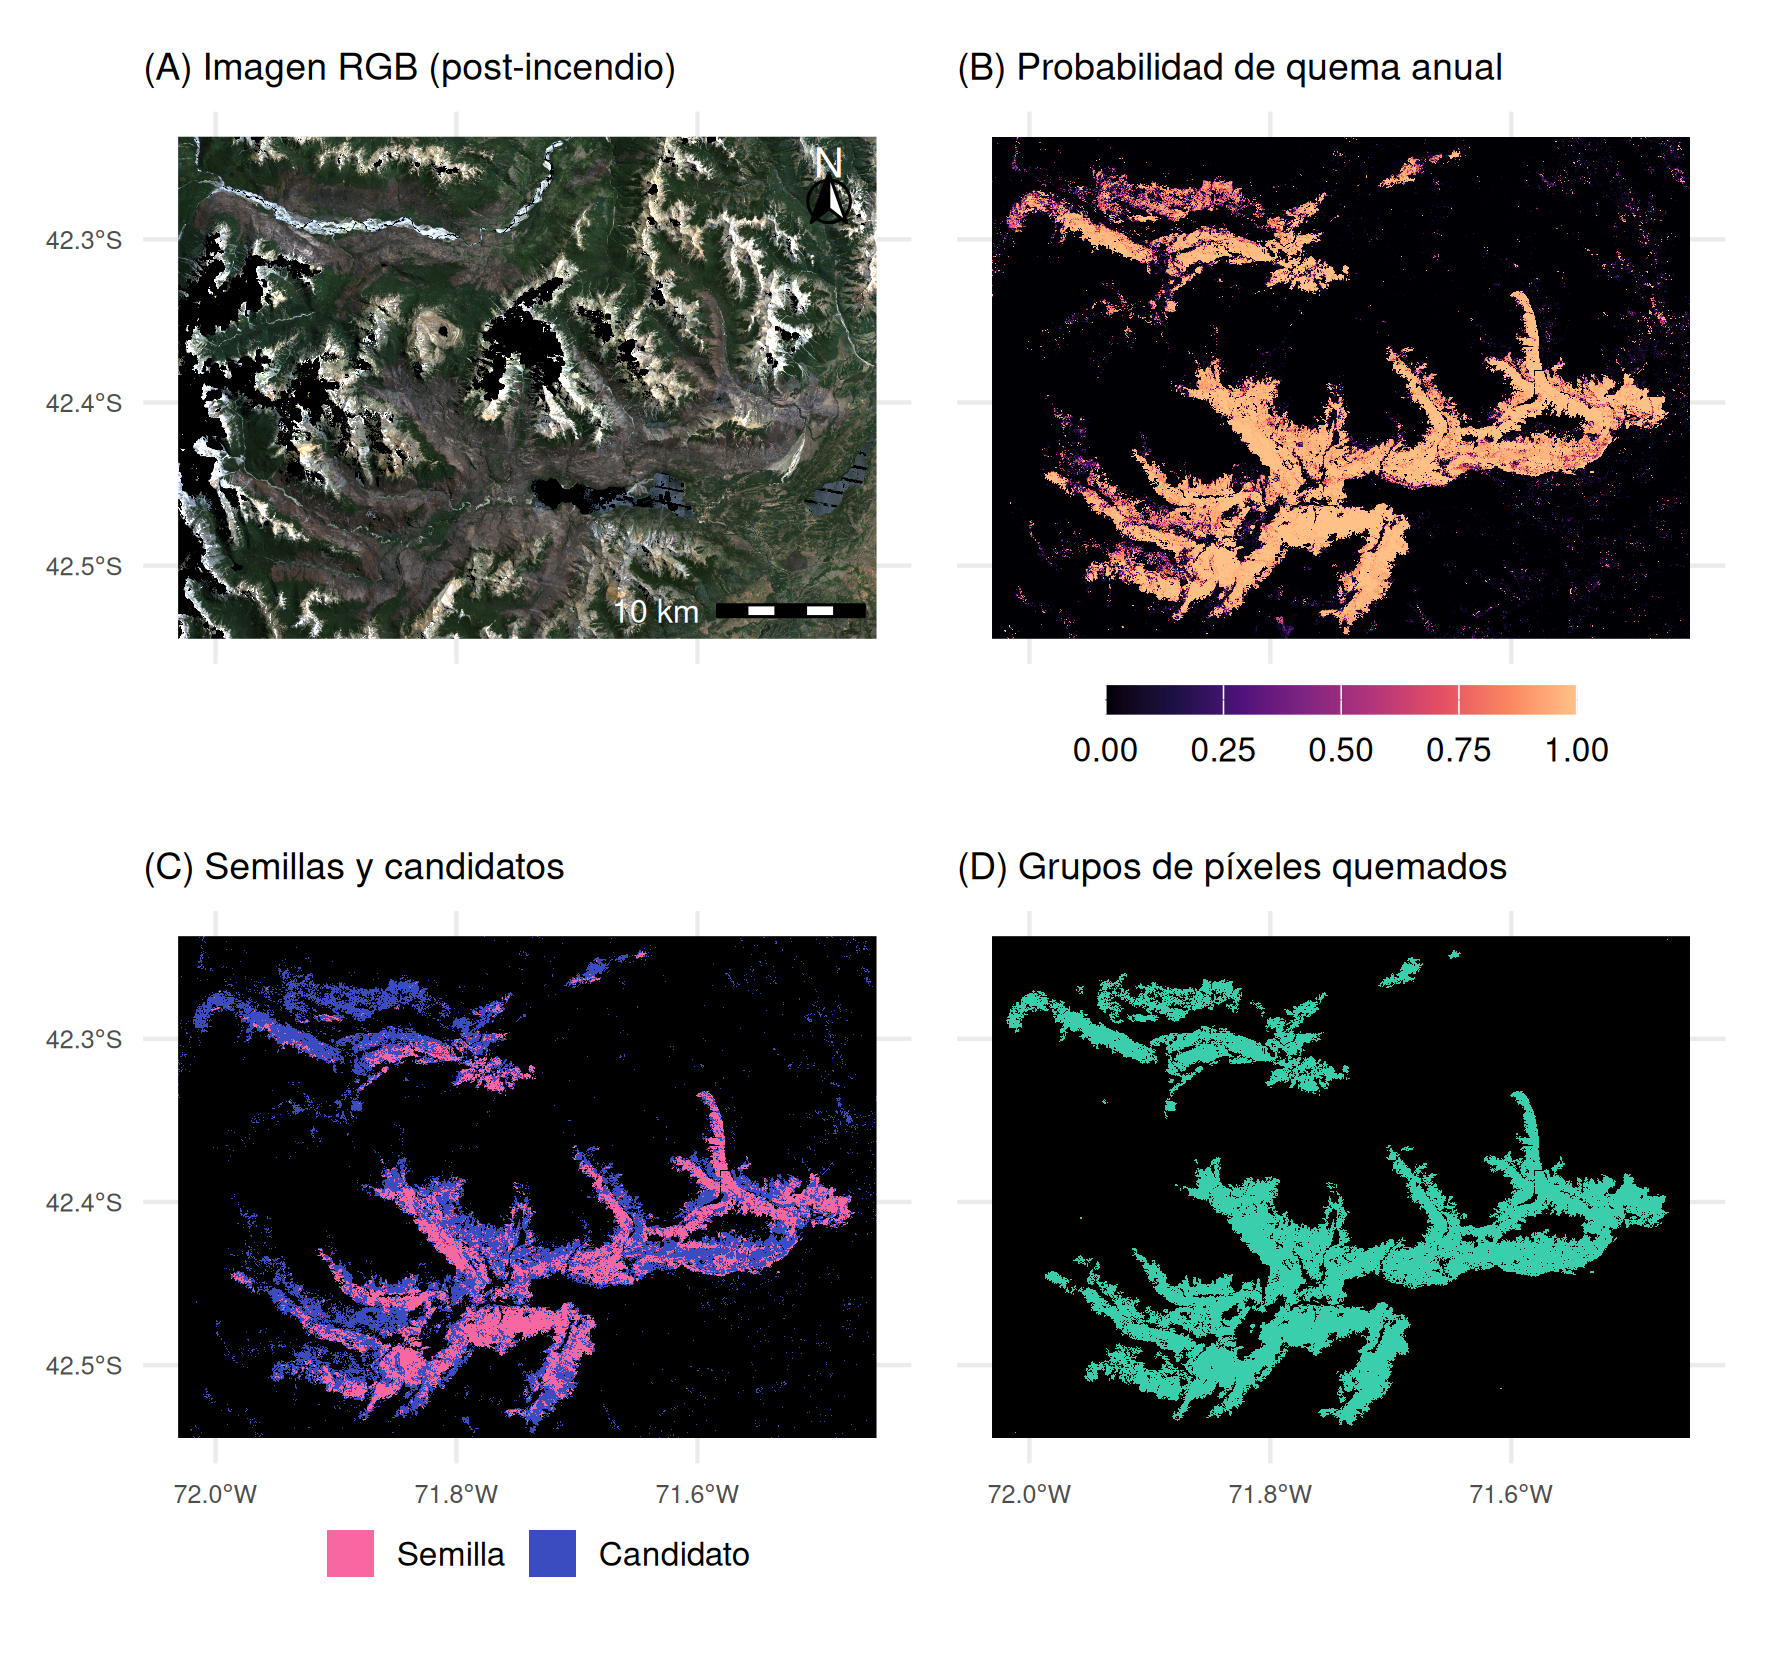
\includegraphics[width=\textwidth]{spatial_analysis.png}
  \caption{Algoritmo de crecimiento de región aplicado a incendios ocurridos en 2015 en la provincia de Chubut: Río Turbio, al norte, y Cholila, al sur. (A) Imagen RGB, correspondiente a la mediana de las imágenes Landsat del verano de 2016, posterior a los incendios, incluída sólo con fines ilustrativos. Las zonas negras corresponden a áreas enmascaradas por los filtros de calidad. (B) Probabilidad de quema a nivel anual, predicha por el modelo. (C) Semillas y candidatos. (D) Resultado del algoritmo de crecimiento de región, mostrando los grupos de píxeles retenidos.}
  \label{fig-region-growing}
\end{figure}

\FloatBarrier

\subsubsection{Definición manual de máscaras}

Los grupos de celdas quemadas obtenidos mendiante el algoritmo de crecimiento de región ayudaron a eliminar una gran parte de falsos positivos, pero aún así, encontramos que el depósito de cenizas volcánicas y zonas esteparias afectadas por sequía eran mapeados como áreas quemadas. Si bien estos fenómenos podrían separarse con filtros a nivel de objetos, dichos filtros generaban errores de omisión. Por ser problemas que ocurrían en años y regiones bien definidas, preferimos excluir esas áreas-momentos del mapeo mediante polígonos de filtrado definidos manualmente.

\subsubsection{Filtrado a nivel de objetos}

Una vez obtenidos los grupos de píxeles con el algoritmo de crecimiento de región, vectorizamos dichos grupos y aplicamos filtros a nivel de objetos para eliminar falsos positivos. En cada polígono calculamos métricas de resumen a partir de capas ráster y métricas de forma. 

A partir de la capa anual de quema, en formato ráster, definimos $\mathrm{burned\_around}_3$ como la proporción de celdas quemadas en un vecindario cuadrado de tres píxeles de radio (ventana de 7 $\times$ 7 píxeles). Esta métrica indica la densidad de la capa de quema, tomando valores bajos en polígonos ralos que suelen ser falsos positivos. A nivel de polígono, esta métrica se resume con el promedio en todos los píxeles incluidos en cada polígono.

Las métricas de forma utilizadas fueron las siguientes:

\[
\begin{aligned}
\mathrm{convexity} &=
\frac{A}{A_{\mathrm{hull}}}, \\[6pt]
\mathrm{shape\_index} &=
\frac{P}{2 \sqrt{\pi A}}, \\[6pt]
\mathrm{circularity} &=
\frac{4 \pi A}{P^2},
\end{aligned}
\]

\noindent donde $A$ es el área del polígono ($\text{m}^2$), $P$ su perímetro ($\text{m}$), y $A_{\mathrm{hull}}$ el área de la envolvente convexa del polígono.

Redefiniendo $A$ como el área en hectáreas, los polígonos fueron retenidos si cumplían las siguientes condiciones:

Polígonos pequeños
\[
\begin{cases}
1 \le A < 50 \\
\mathrm{burned\_around}_3 > 0.7 \\
\mathrm{convexity} > 0.5 \\
\mathrm{shape\_index} < 7 \\
\mathrm{circularity} > 0.01
\end{cases}
\]

Polígonos medianos
\[
\begin{cases}
50 < A \le 300 \\
\mathrm{burned\_around}_3 > 0.6 \\
\mathrm{convexity} > 0.4 \\
\mathrm{shape\_index} < 7
\end{cases}
\]

Todos los polígonos mayores a 300 ha fueron retenidos.

Nótese que ningún polígono menor a 1 ha fue retenido, siendo esta la mínima unidad mapeable.

\subsection{Postprocesamiento}

Una vez filtrados los polígonos, generamos las capas ráster anuales de área quemada. Como el algoritmo de mapeo duplica las áreas quemadas al comienzo o fin de cada año calendario, inicialmente removimos los duplicados. Utilizamos como fecha de quema date\_mid, definida más arriba. En cada año, generamos una máscara que mantenía sólo las áreas incluidas en los polígonos filtrados correspondientes al año focal y los píxeles cuyo date\_mid correspondía al año focal. De esta manera, para incendios que transcurren entre diciembre y marzo, toda su área es analizada en conjunto en el bloque de análisis espacial, pero el producto final de MapBiomas lo muestra separado en las capas de dos años consecutivos.

Para obtener el mes de quema, transformamos date\_mid de año fraccional a mes.

Para obtener el tamaño de la cicatriz ejecutamos el algoritmo \texttt{connectedComponents} de GEE en dichas capas anuales filtradas por fecha.

\section{Productos generados}

Generamos dos \textit{assets} de GEE: 

\begin{itemize}
  \item \texttt{burned\_area\_annual}: \texttt{ImageCollection} con una imagen por año, en donde cada imagen consta de dos bandas: \texttt{month}, con el mes de quema, y \texttt{scar\_size}, con el tamaño de la cicatriz. Cada imagen cuenta con la propiedad \texttt{year} para su filtrado.
  \item \texttt{fire\_freq}: imagen con dos bandas: \texttt{freq}, con la cantidad de años en que se quemó cada píxel, y \texttt{last}, indicando en qué año ocurrió el incendio más reciente. 
\end{itemize}

Los productos pueden visualizarse en este \href{https://code.earthengine.google.com/b9bf25f7ffff974ed79a6c262e84f65e}{enlace}, utilizando el Editor de Código de GEE.

\section{Reproducibilidad}

El código y la documentación necesaria para reproducir este flujo de trabajo se encuentran alojados en \href{https://github.com/barberaivan/mapbiomas-argentina-fire}{GitHub}.

\section{Desafíos encontrados}

Si bien este piloto no cuenta con un análisis de validación, notamos que en general el algoritmo presenta un notable error de comisión, mientras que el error de omisión es relativamente bajo. 

Los errores de comisión de mayor extensión espacial estuvieron asociados a una sequía en una región esteparia situada al norte del área de estudio, ocurrida en 2015, y al depósito de cenizas volcánicas asociadas a la erupción del complejo volcánico Puyehue-Cordón Caulle en 2011, que abarcó cerca de la mitad del área de estudio. Estas alteraciones en la reflectancia presentan cambios en la señal espectral similares a los que genera el paso del fuego, si consideramos los índices analizados NBR, NBR2, MIRBI y NDVI. Sin embargo, presentan algunas características distintivas. 

La sequía de 2015 se diferencia de las áreas quemadas por la velocidad del cambio: mientras que el fuego genera una caída abrupta en los índices analizados, la sequía tiende a generar un cambio gradual. Si la densidad de imágenes es alta, como en 2015, se puede notar que las diferencias máximas consecutivas en probabilidad de quema (pdiff\_max) tienden a ser más bajas que en una zona quemada. Aplicando un criterio de elevada pdiff\_max para las semillas en el algoritmo de crecimiento de región, muy pocos píxeles afectados por sequía cumplen esta condición. Sin embargo, sequías ocurridas en períodos con baja densidad de imágenes pueden presentar valores de pdiff\_max elevados, ya que esta diferencia en probabilidad no considera la separación temporal entre observaciones, sólo su orden. Con nuestra definición de semillas, el algoritmo de crecimiento de región generó grupos de píxeles grandes y con muy baja densidad de semillas en la zona afectada por sequía.

Las cenizas volcánicas se separaban con mayor facilidad de las áreas quemadas en base a información espectral, ya que las mismas presentaban un brillo elevado. Imponiendo restricciones de brillo sobre las semillas, una baja proporción de píxeles cubiertos por ceniza pasaban ese filtro. Nuevamente, el algoritmo de crecimiento de región generó grandes grupos de píxeles con baja densidad de semillas en la zona cubierta por ceniza volcánica. 

En base a estas características propias de las zonas afectadas por sequía y cenizas, intentamos separar estos grupos de píxeles de los correspondientes a áreas quemadas mediante métricas a nivel de objetos. El primer candidato fue la densidad de semillas del polígono. Sin embargo, encontramos que algunos incendios de estepa, particularmente al comienzo de la serie (1999-2002) también tenían baja densidad de semillas, con lo cual, establecer umbrales con esta variable para filtrar falsos positivos generaba errores de omisión. Por la naturaleza localizada en el tiempo y el espacio de la sequía y el depósito de cenizas, preferimos quitar los polígonos asociados manualmente. Sin embargo, a futuro sería deseable implementar un filtro automático, basado en un modelo, para reducir la carga de trabajo manual.

Aparte de estos errores de comisión de gran extensión, encontramos una gran cantidad de polígonos pequeños que no parecen estar asociados a fuego. En la gran mayoría de los casos, estos fueron polígonos ralos, altamente ramificados, que pudieron eliminarse con filtros de forma y densidad a nivel de objetos. Sin embargo, estos filtros no resuelven el problema completamente. En algunos casos, estos errores de comisión estaban asociados a otros disturbios, como deforestación y defoliaciones por insectos, o a actividad agrícola. 

\section{Líneas prioritarias de mejora}

A continuación mencionamos los aspectos a mejorar en la metodología que consideramos tendrían un efecto notable en la precisión del mapeo, intentando listarlos según influencia decreciente. Aquí no consideramos la inclusión de información provista por otros sensores remotos aparte de Landsat, ya que para las primeras colecciones apuntaremos a refinar el mapeo sin comprometer la extensión temporal del producto.

\subsection{Datos de entrenamiento contemplando falsos positivos}

Independientemente del paso del algoritmo que se considere, creemos que utilizar datos relacionados a otros disturbios que generan cambios espectrales similares al fuego será clave para mejorar el algoritmo. Estos datos pueden utilizarse para diseñar filtros y/o para ajustar modelos (los filtros pueden ser considerados modelos sencillos). Sin embargo, un desafío considerable es colectar datos de otros disturbios, ya que los mismos varían entre regiones (agricultura, sequías, inundaciones, tala, cenizas, etc.) y su extensión espacial y temporal a veces es reducida. 

Por otro lado, dado que en muchos casos estos procesos presentan una señal espectral similar a la de áreas quemadas, definir la cantidad relativa de observaciones de cada disturbio para entrenar un modelo resulta de gran importancia. A menor separabilidad de clases, mayor es el efecto de la abundancia relativa de las clases en el conjunto de entrenamiento.

\subsection{Clasificación a nivel de objetos mediante un modelo}

Los filtros a nivel de objetos pueden ser reemplazados o complementados con un clasificador a nivel de objetos. Además de las variables de forma, densidad y tamaño ya utilizadas, sería conveniente también considerar la proporción de semillas, el promedio de pdiff\_max, y la proporción de cada tipo de vegetación en el año previo. Análisis exploratorios sugieren que la clase del polígono (incendio vs. falso positivo) no responde linealmente a estas variables, con lo cual sería conveniente utilizar un modelo flexible. A su vez, ajustar y evaluar el modelo fuera de GEE sería plausible, ya que el mismo sólo utilizaría la tabla de atributos de los polígonos, lo cual no requiere exportar y procesar un gran volumen de datos. Por este motivo se podrían utilizar modelos complejos y costosos no disponibles en GEE, como redes neuronales.

\subsection{Clasificador a nivel de observación}

El modelo a nivel de observación puede ser mejorado sustancialmente utilizando más índices espectrales o bandas, y, eventualmente, incluyendo datos sobre otros disturbios. La regresión logística podría extenderse a una regresión categórica (regresión multinomial de tamaño 1), la cual predice la probabilidad de muchas clases, por ejemplo: no quemado, quemado, nube, agua, ceniza, deforestación-defoliación, agricultura, sequía. Una alternativa es generar modelos separados accesorios sencillos, por ejemplo, un modelo que prediga la probabilidad de nube/nieve/hielo basado únicamente en el brillo, y multiplicar la probabilidad de quema por la probabilidad de no-[nube/nieve/hielo]. 

Dado que este modelo debe predecir la probabilidad de cada clase en todas las imágenes Landsat que intersectan el área y período de interés, el mismo debería poder implementarse en GEE para aprovechar su capacidad de cómputo. Con esta consideración, quizás las opciones deban limitarse a regresión logística/categórica y random forest.

\subsection{Definición de semillas y candidatos}

La definición de estas capas puede alterar en gran medida los resultados obtenidos. En particular, estableciendo criterios estrictos para semillas que difícilmente se alcancen con disturbios no relacionados a fuego puede generar una baja densidad de semillas en polígonos resultantes de estos disturbios.

\subsection{Suavizado y resumen de series temporales}

Suavizar la serie temporal de probabilidad de quema utilizando un número de observaciones dinámico para calcular la mediana podría mejorar la precisión. Series con baja densidad de imágenes podrían utilizar $K=3$ en vez de $K=5$, y series ruidosas con alta densidad de imágenes podrían utilizar $K=7$. 

A su vez, las series temporales podrían resumirse incluyendo métricas de velocidad de cambio, tanto en el aumento de la probabilidad de quema como en su disminución. Esto ayudaría a diferenciar cambios graduales (e.g., sequía) de cambios abruptos (posiblemente fuego).

\section{Consideraciones para la Colección 1}

El objetivo de la Colección 1 es extender el mapeo de áreas quemadas a toda la Argentina y al periodo 1985-2025. Durante dicha Colección, y probablemente en algunas más, nos limitaremos a utilizar únicamente imágenes Landsat. El algoritmo aquí descrito se ejecutará de forma separada para las cinco regiones definidas por MapBiomas Argentina: Patagonia; Monte, Puna y Altos Andes; Chaco; Pampas, y Bosque Atlántico. Para cada región tomaremos un volumen de muestras similar al utilizado en este piloto, de forma que los modelos serán estimados región por región. Para mapear áreas quemadas en el primer año de la serie ajustaremos modelos accesorios que sólo utilizarán información del año focal, ya que el año previo no está disponible.  

Probablemente el mayor desafío sea separar áreas quemadas de otros procesos de cambio, como inundaciones, agricultura, tala, sequías, así como detectar incendios de sotobosque en las regiones más productivas. Sin embargo, estos desafíos y sus soluciones variarán entre regiones. Ante esta situación, nos proponemos seguir el mismo procedimiento aquí descrito pero con una reevaluación a mitad de camino: tras obtener los mapas de probabilidad de quema anual podremos evaluar visualmente los mayores problemas en cada región. A partir de allí analizaremos la factibilidad de implementar algunas de las mejoras mencionadas arriba. Dado el bajo costo de tomar datos a nivel de objetos, es probable que en la Colección 1 optemos por esa estrategia.

Para la Colección 1 priorizamos extender el mapeo a toda la Argentina y al período 1985-2025, y tomar datos a fin de generar un producto de calidad razonable. Debido a restricciones temporales, no planeamos realizar un análisis de validación del producto, el cual está previsto para la Colección 2, que se lanzará en 2027.

Respecto a la toma de datos de entrenamiento para estimar los modelos de probabilidad de quema a nivel de observación y anual, planeamos seguir el mismo esquema en Monte, Puna y Altos Andes, en Chaco y en Pampas. En Bosque Atlántico muestrearemos $20$ incendios, no $30$, por la menor extensión de la región. En Patagonia agregaremos $15$ incendios más, para cubrir la zona sur y este. Suponemos que el tiempo promedio de recolección de incendios en las demás regiones será un $50$ \% mayor, debido a la mayor frecuencia de fuegos, lo que requiere mayor cuidado para evitar superposiciones.

Bajo estas consideraciones, podemos estimar el tiempo requerido para tomar las muestras necesarias para la Colección 1. Para recolectar un incendio, se requieren $5.1 / 30 \times 1.5 = 0.255$~h. Para agregar $30 \times 3 + 20 + 15 = 125$ incendios, se requerirán $0.255 \times 125 = 31.88$~h de recolección de incendios. Suponiendo que el tiempo de recolección de muestras en cada incendio toma lo mismo que tomó en este piloto ($35.97$~h para $12889$ puntos, $35.97 / 12889 = 0.00279$~h por punto), y tomando 400 puntos por incendio ($200$ quemado y $200$ no quemado), se requerirán $0.00279 \times 400 \times 125 = 139.50$~h para la recolección de muestras. En total, se requerirán $31.88 + 139.50 = 171.38$~h para tomar las muestras necesarias para la Colección 1, lo que equivale a $21.42$ días laborales de $8$~h.

Idealmente, se podría destinar un esfuerzo equivalente a tomar datos de otros disturbios, y alrededor de un $50$ \% de este tiempo a tomar datos a nivel de objetos (esto requiere menos esfuerzo). En total, se podría requerir un esfuerzo de alrededor de $171.38 \times 2.5 = 428.45$ h para tomar todos los datos necesarios para la Colección 1.

Suponiendo que 

\begin{itemize}
  \item el mismo tiempo se requiere para desarrollar y ejecutar el algoritmo completo, considerando las mejoras propuestas y adaptaciones necesarias,
  \item se requiere un $40$ \% de ese tiempo para desarrollar la documentación del producto (ATBD y repositorio de GitHub) y llevar a cabo un análisis preliminar de los resultados para dar a conocer el producto, y que 
  \item la Ley de Hofstadter indica que todo lleva más tiempo de lo esperado, incluso si se tuvo en cuenta la Ley de Hofstadter \parencite{hofstadter1979}, por lo que inflamos el tiempo total en un factor de $1.1$\footnote{Nótese que no tomamos esta ley tan en serio, ya que ello nos llevaría a una recursión infinita, en cuyo límite el tiempo requerido tendería a $\infty$~h.},
\end{itemize}

\noindent el esfuerzo total para lanzar la Colección 1 sería de $428.45 \times (2 + 0.4) \times 1.1 = 1131.11$ h. Considerando que los \textit{assets} de la Colección 1 deben estar disponibles el 1ro de julio de 2026, y suponiendo que contaremos con tres contratos anuales de $10$ h semanales cada uno (total $3 \times 10 \times 52 = 1560$ h), el plan de trabajo resulta plausible. El tiempo de trabajo del personal contratado debería concentrarse principalmente en la primera mitad del año, pero dado que contamos, además, con técnicos voluntarios, eso podría no ser necesario. 

%\section{[Tareas (para completar este documento)]}

%- Incluir figura de series temporales (spaghetti plot et al.) y citarla debidamente a lo largo de la explicación.
%- Incluir figura de SNIC y citarla.
%- Documentar y actualizar GitHub.
%- Actualizar código de ejemplo cuando estén los assets.


\newpage

\printbibliography

\end{document}